\chapter{Smoothing Delay} 
\lstset{style=6502Style}

\begin{figure}[H]
    \centering
    \begin{adjustbox}{width=10.5cm,margin=0cm}
      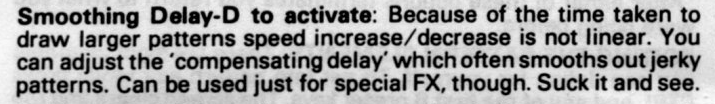
\includegraphics[width=12cm]{src/delay/manual-entry.png}%
    \end{adjustbox}
    \caption{
      Excerpt from Manual (Part No. LC1982-Vb). Smoothing Delay.
      }
\end{figure}

\begin{lstlisting}[caption=From \icode{CheckKeyboardInput}.]
MaybeDPressed   
  CMP #KEY_D ; 'D' pressed?
  BNE MaybeCPressed

  ; Smoothing Delay, D to activate: Because of the time taken to draw
  ; larger patterns speed increase/decrease is not linear. You can adjust
  ; the 'compensating delay' which often smooths out jerky patterns. Can
  ; be used just for special FX, though. Suck it and see.
  LDA #SMOOTHING_DELAY
  STA currentVariableMode
  RTS 
\end{lstlisting}
\begin{figure}[H]
    \centering
    \begin{adjustbox}{width=3cm,margin=11cm -12cm}
      
\includegraphics[width=12cm]{src/delay/delay-low.png}%
    \end{adjustbox}
    \begin{adjustbox}{width=10.5cm,center}
      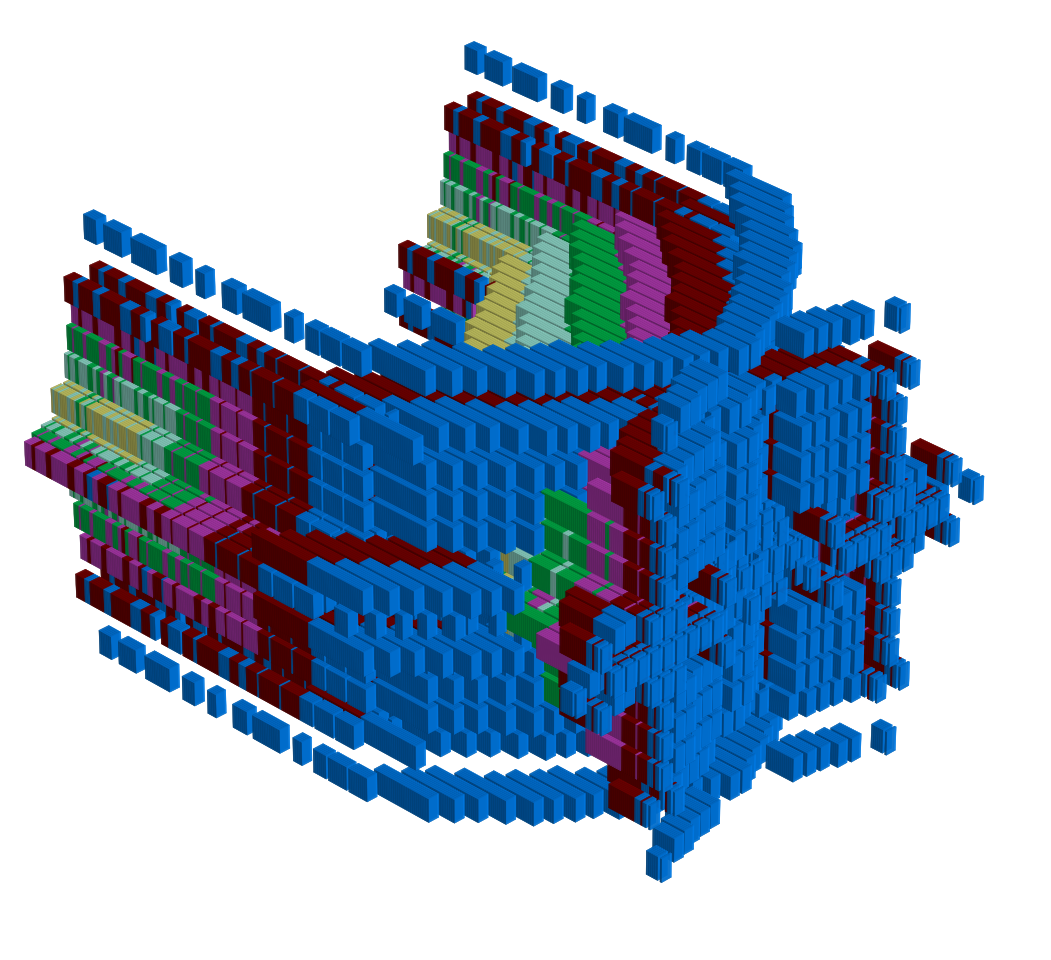
\includegraphics[width=12cm]{src/delay/pattern0-45.png}%
    \end{adjustbox}
    \begin{adjustbox}{width=3cm,margin=11cm -12cm}
      
\includegraphics[width=12cm]{src/delay/delay-high.png}%
    \end{adjustbox}
    \begin{adjustbox}{width=10.5cm,margin=0cm -2cm}
      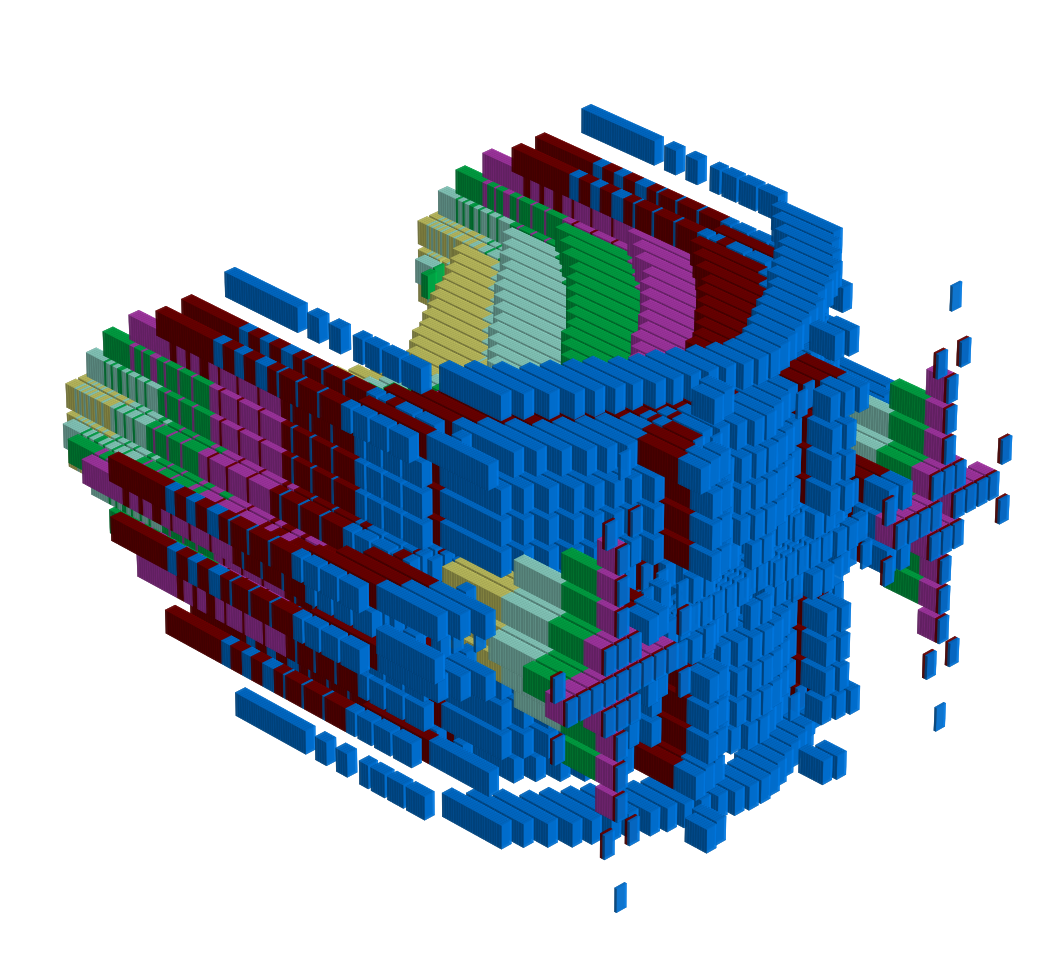
\includegraphics[width=12cm]{src/delay/pattern1-45.png}%
    \end{adjustbox}
    \caption{Effect of low and high values for Smoothing Delay}
\end{figure}
                                                                           
\begin{lstlisting}[caption=From \icode{MainInterruptHandler}.]
ApplySmoothingDelay    
        LDA smoothingDelay
        STA initialFramesRemainingToNextPaintForStep,X
        STA framesRemainingToNextPaintForStep,X
\end{lstlisting}

\begin{lstlisting}[caption=Definition of \icode{framesRemainingToNextPaintForStep} and its counterpart \icode{initialFramesRemainingToNextPaintForStep}..]
initialFramesRemainingToNextPaintForStep
        .BYTE $00,$00,$00,$00,$00,$00,$00,$00
        .BYTE $00,$00,$00,$00,$00,$00,$00,$00
        .BYTE $00,$00,$00,$00,$00,$00,$00,$00
        .BYTE $00,$00,$FF,$FF,$FF,$FF,$FF,$FF
        .BYTE $FF,$FF,$FF,$FF,$FF,$FF,$FF,$FF
        .BYTE $FF,$FF,$FF,$FF,$FF,$FF,$FF,$FF
        .BYTE $FF,$FF,$FF,$FF,$FF,$FF,$FF,$FF
        .BYTE $FF,$FF,$FF,$FF,$FF,$FF,$FF,$FF
framesRemainingToNextPaintForStep
        .BYTE $FF,$FF,$FF,$FF,$FF,$FF,$FF,$FF
        .BYTE $FF,$FF,$FF,$FF,$FF,$FF,$FF,$FF
        .BYTE $FF,$FF,$FF,$FF,$FF,$FF,$FF,$FF
        .BYTE $FF,$FF,$FF,$FF,$FF,$FF,$FF,$FF
        .BYTE $FF,$FF,$FF,$FF,$FF,$FF,$FF,$FF
        .BYTE $FF,$FF,$FF,$FF,$FF,$FF,$FF,$FF
        .BYTE $FF,$FF,$FF,$FF,$FF,$FF,$FF,$FF
        .BYTE $FF,$FF,$FF,$FF,$FF,$FF,$FF,$FF
\end{lstlisting}


\begin{lstlisting}[caption=From \icode{MainPaintLoop}.]
ShouldDoAPaint   
        STA currentIndexToColorValues
        DEC framesRemainingToNextPaintForStep,X
        BNE GoBackToStartOfLoop

        ; Actually paint some pixels to the screen.

        ; Reset the delay for this step.
        LDA initialFramesRemainingToNextPaintForStep,X
        STA framesRemainingToNextPaintForStep,X

        ; Get the x and y positions for this pixel.
        LDA pixelXPositionArray,X
        STA pixelXPositionZP
        LDA pixelYPositionArray,X
        STA pixelYPositionZP

        LDA patternIndexArray,X
        STA presetIndex

        LDA symmetrySettingForStepCount,X
        STA currentSymmetrySettingForStep

        LDA currentIndexToColorValues
        AND #$80
        BNE ResetAndGoBackToStartOfLoop

        TXA 
        PHA 
        JSR LoopThroughPixelsAndPaint
        PLA 
        TAX 
\end{lstlisting}
\clearpage
\begin{figure}[H]
    \centering
    \begin{adjustbox}{width=10.5cm,margin=0cm}
      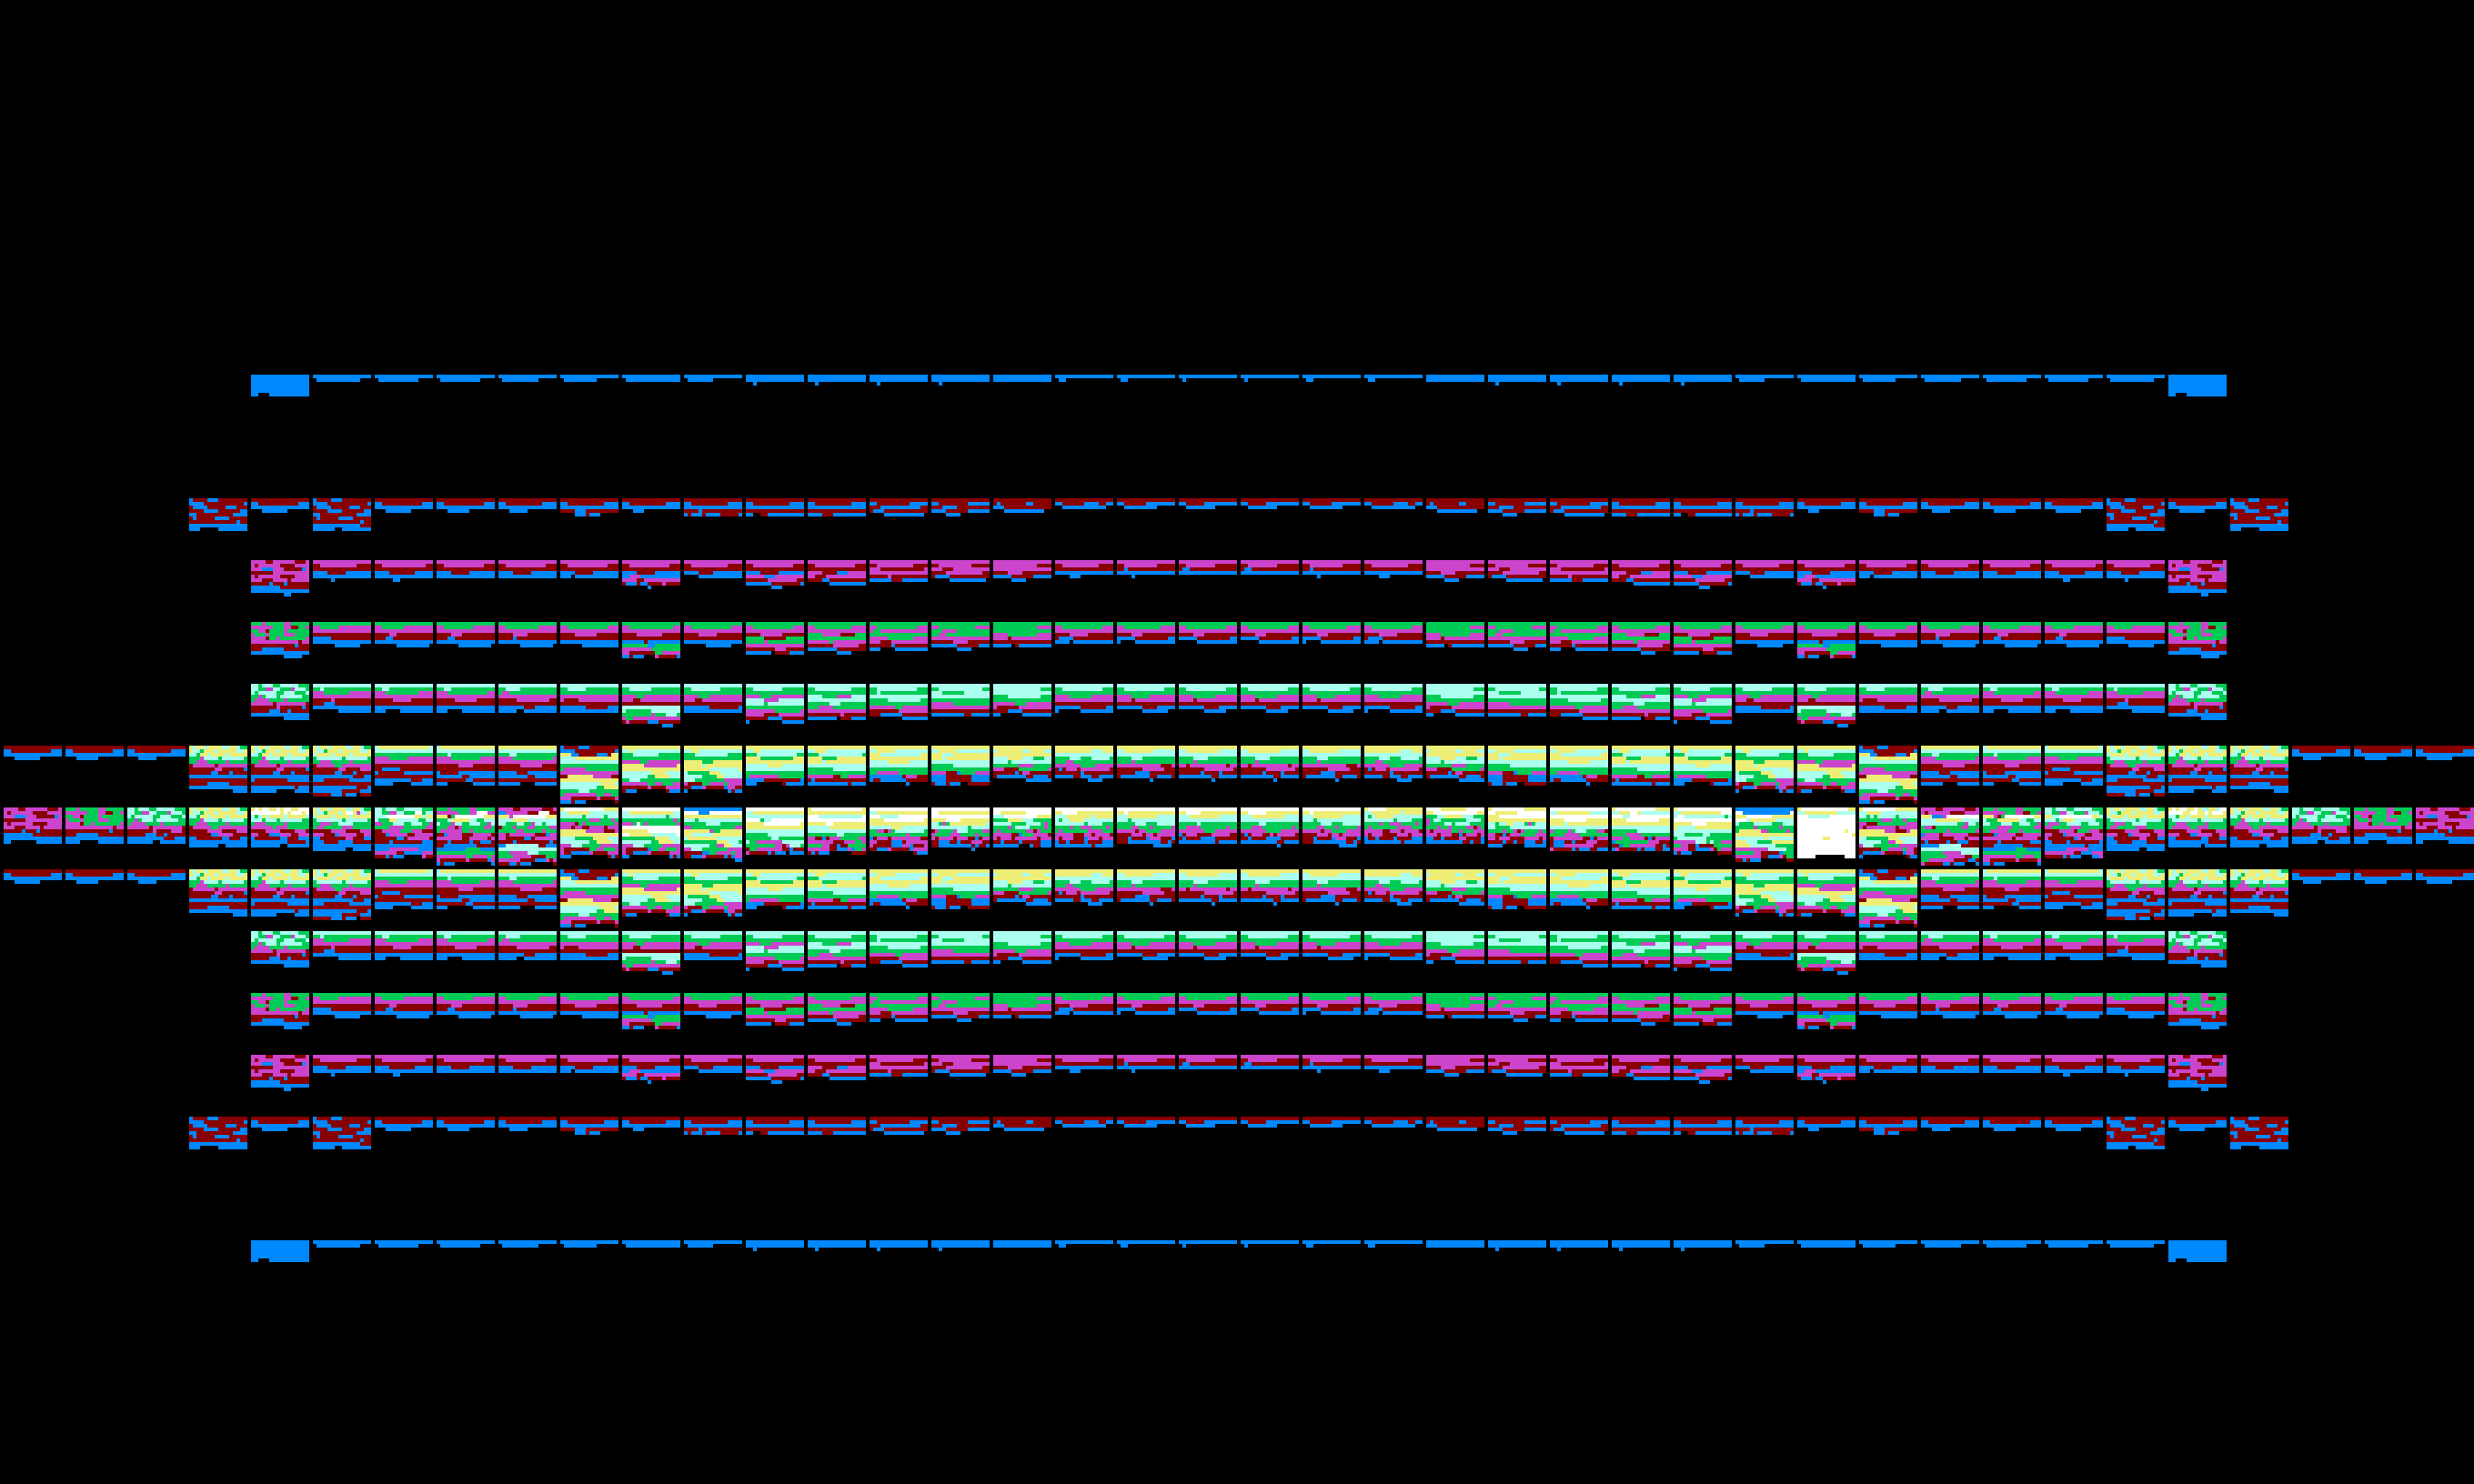
\includegraphics[width=12cm]{src/delay/pixelhist-0.png}%
    \end{adjustbox}
    \caption{
      
\includegraphics[width=4cm]{src/delay/delay-low.png}%
      }
\end{figure}
\begin{figure}[H]
    \centering
    \begin{adjustbox}{width=10.5cm,margin=0cm}
      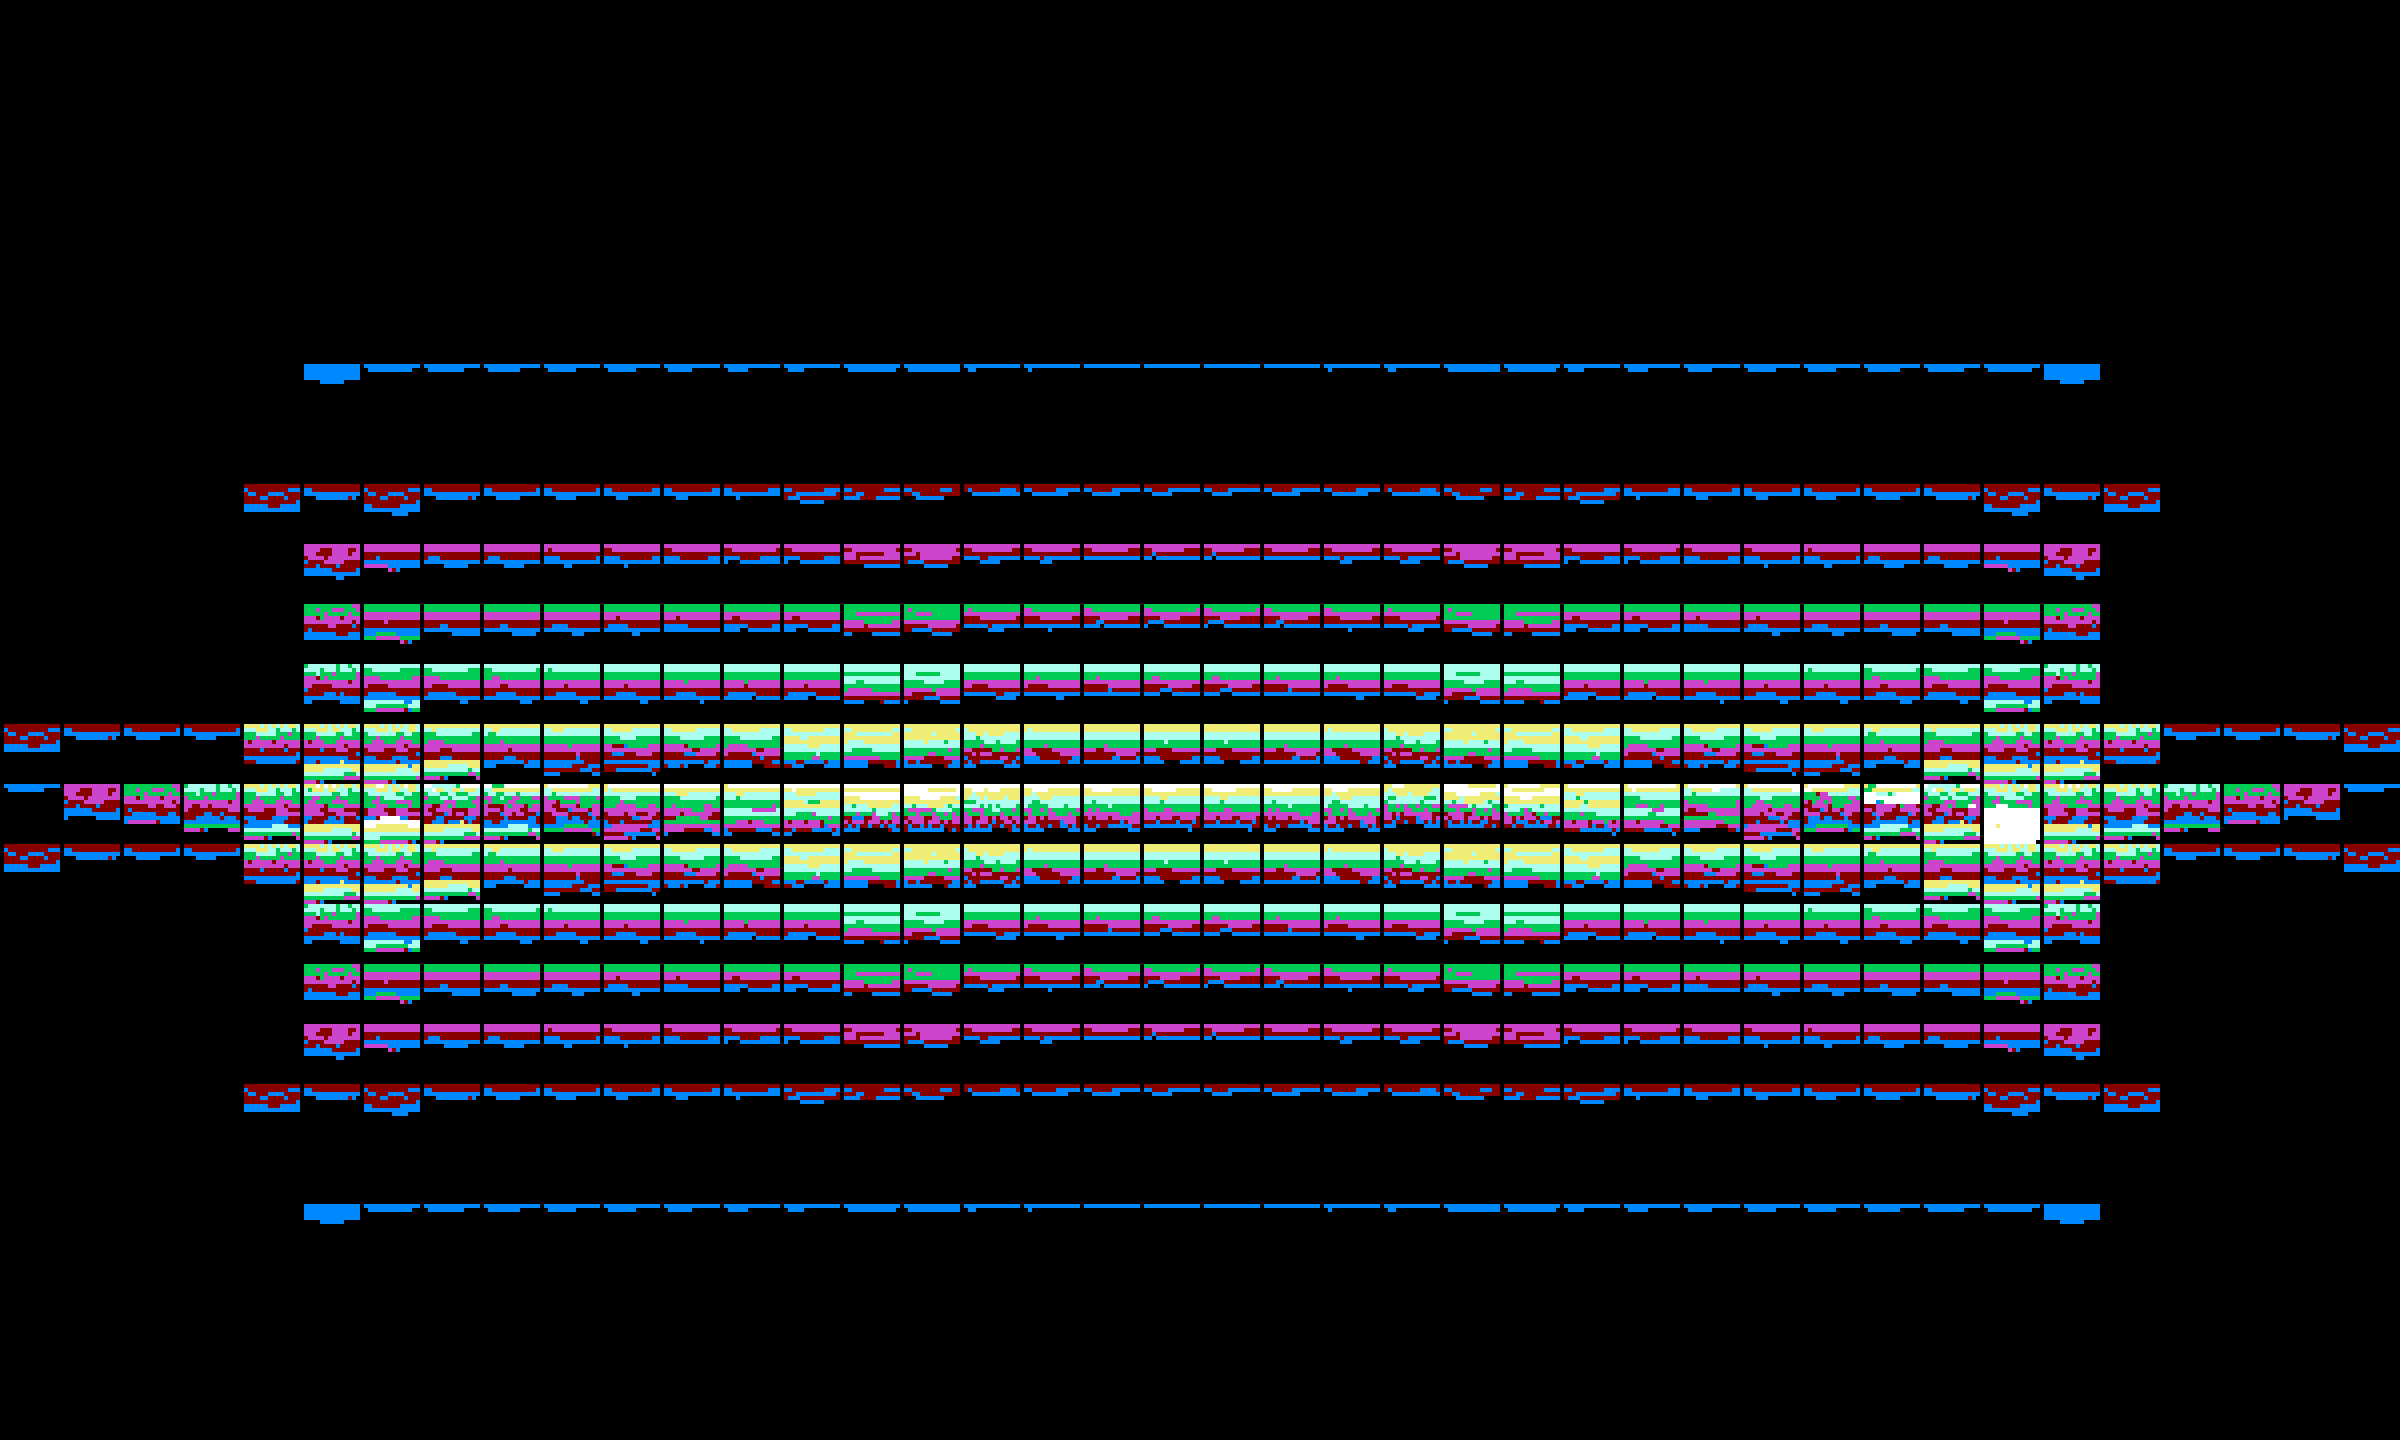
\includegraphics[width=12cm]{src/delay/pixelhist-1.png}%
    \end{adjustbox}
    \caption{
      
\includegraphics[width=4cm]{src/delay/delay-high.png}%
      }
\end{figure}
